%===================================== CHAP 2 =================================

\chapter{PCB design procedure}
This chapter explains the workflow used to create the PCB prototype in Eagle and visualize it into a 3D model using Fusion 360. 
Three parts are necessary to create a PCB in eagle:
\begin{enumerate}
\item The schematics which is a diagram with electrical connections to the different components in the circuit.  
\item The board shows the physical representation of the electrical connections between the different components
\item The library contains the components used to create both the schematics (diagrams) and board (footprint).
\end{enumerate}

We start by creating a new project by adding a new folder under projects and add all of the 3 parts above.
This is done by clicking on File $\rightarrow$ New $\rightarrow$ then choosing the three options above. 

\begin{figure}[h]
\begin{center}
\center
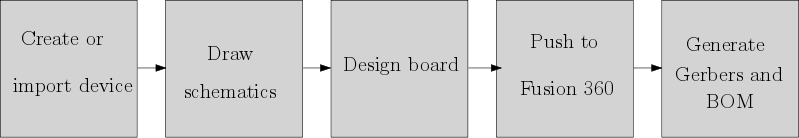
\includegraphics[scale=0.5]{Illustrations/workflow.png}  
\caption{Design workflow in Eagle}
\label{block diagram}
\end{center}
\end{figure}

\section{EAGLE’s schematics}
In order to draw the schematics, the right components must be found or created.  Standard components like capacitors, resistors, voltage sources and ground can be found in standard libraries and can easily be imported to a library or used in the schematics. The full board schematics is shown in Appendix \ref{Full_schematics}. 


\subsection{Creating a component in Eagle}
Eagle's component logic is \textbf{Symbol + Package = Device.} These three parts are described and created for the RF430CL330H chip.

\begin{enumerate}
\item The symbol will be shown on the schematics.
\item The package contain the footprint of the component and will be shown in the board.
\item The device combines both the symbol and package into one component.
\end{enumerate} 


\subsection{Creating the Symbol}
The datasheet for the RF430CL330H \cite{TexasInstruments2012} is used to create a new symbol with correct pin numbers and description. 

\begin{figure}[h]
\begin{center}
\center
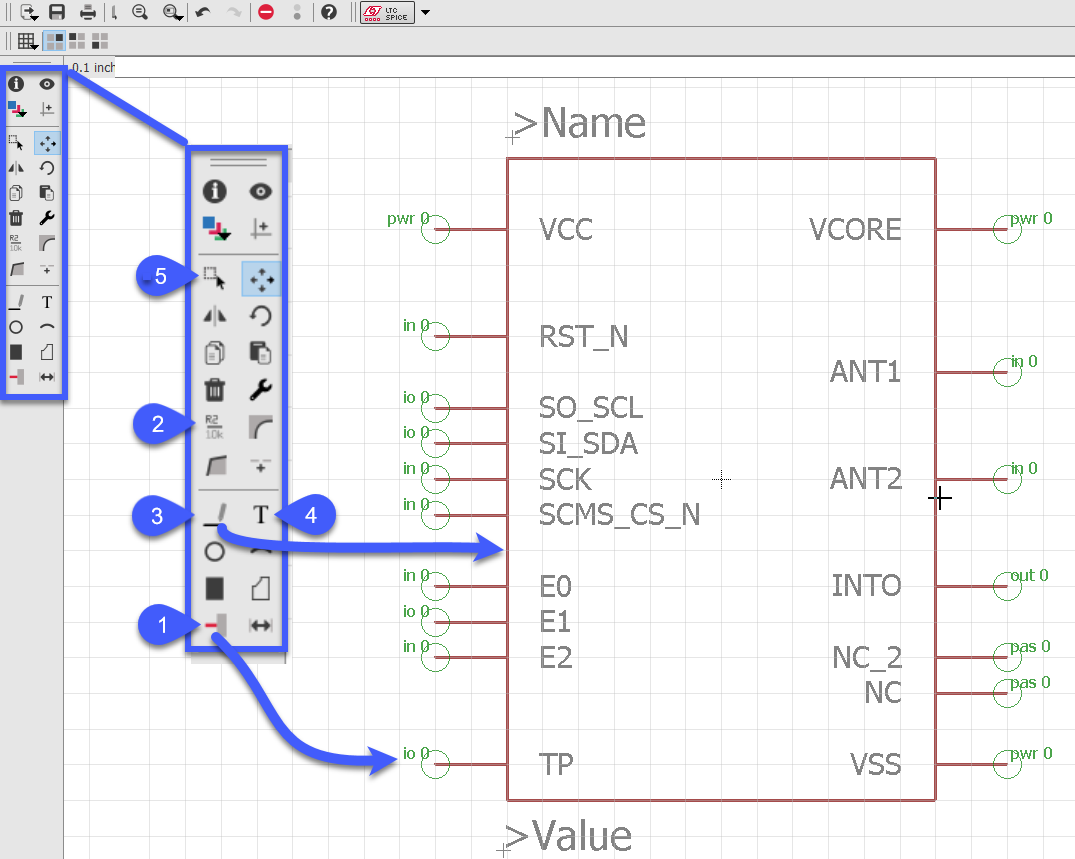
\includegraphics[scale=0.4]{Illustrations/Creating_a_symbol.png} 
\caption{Creating a symbol in eagle}
\label{symbol}
\end{center}
\end{figure}

\begin{enumerate}
\item Add the pins, we can find this information in the datasheet. This chip has 15-pin.
\item Select the name tool to add a name to each pin.
\item Create an outline using the line tool, and move the components as shown in the Figure \ref{symbol}
\item Add text with $>$Name and $>$Value. This will be used later when creating the device.
\item Move the components to the desired positions as shown in step \textbf{(5)} and save.
\end{enumerate}


\subsection{Creating the Package}
In the library editor choose library $\rightarrow$ table of contents. Then add a new package named \textbf{VQFN-16 (RGT)} and follow the steps shown in Figure \ref{creating_package}.
\begin{figure}[h]
\begin{center}
\center
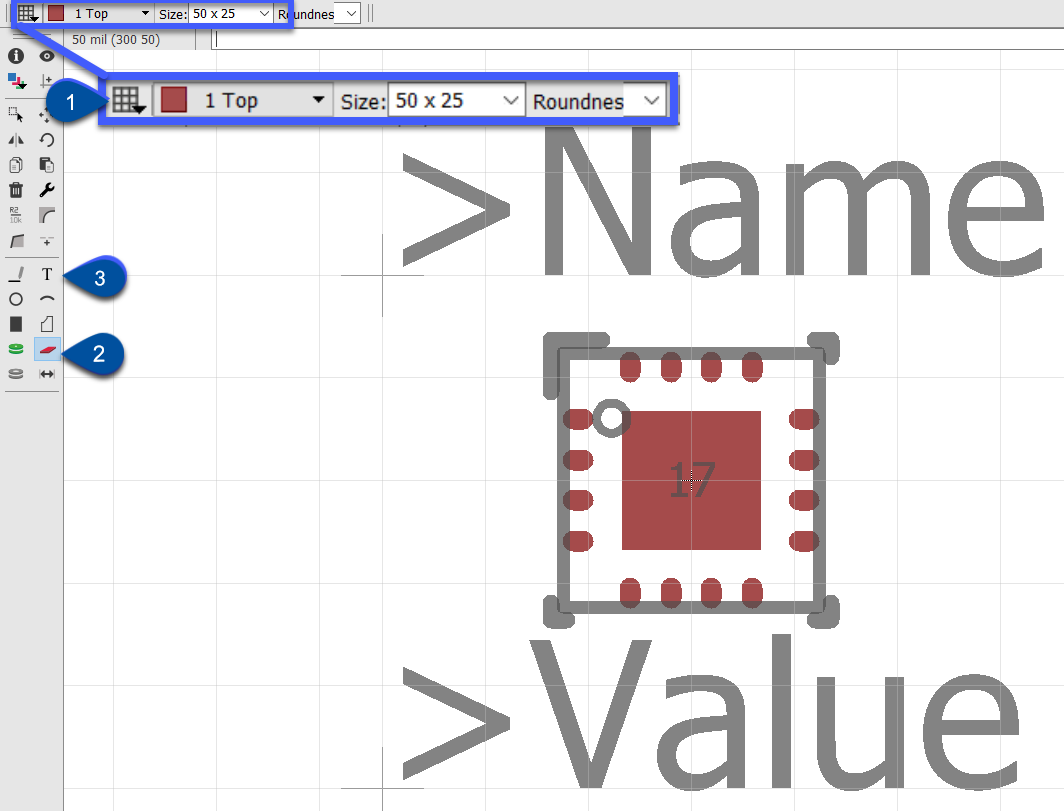
\includegraphics[scale=0.35]{Illustrations/creating_a_package.png} 
\caption{Creating a package in Eagle}
\label{creating_package}
\end{center}
\end{figure}

\begin{enumerate}
\item It's important to choose the right grid size, the correct spacing is given in the datasheet \cite{TexasInstruments2012}. 
\item Choose the SMD tool and add 17 pads to the top layer.
\item Add text $>$Name and $>$Value to layers \textbf{tNames} and \textbf{tValues} respectively. The outline is done using the line tool to the \textbf{tDoc} laye. Save the new footprint.
\end{enumerate}


\subsection{Creating the Device}
In order to create the device we go to the library $\rightarrow$ table of content, then click add device.
\begin{figure}[h]
\begin{center}
\center
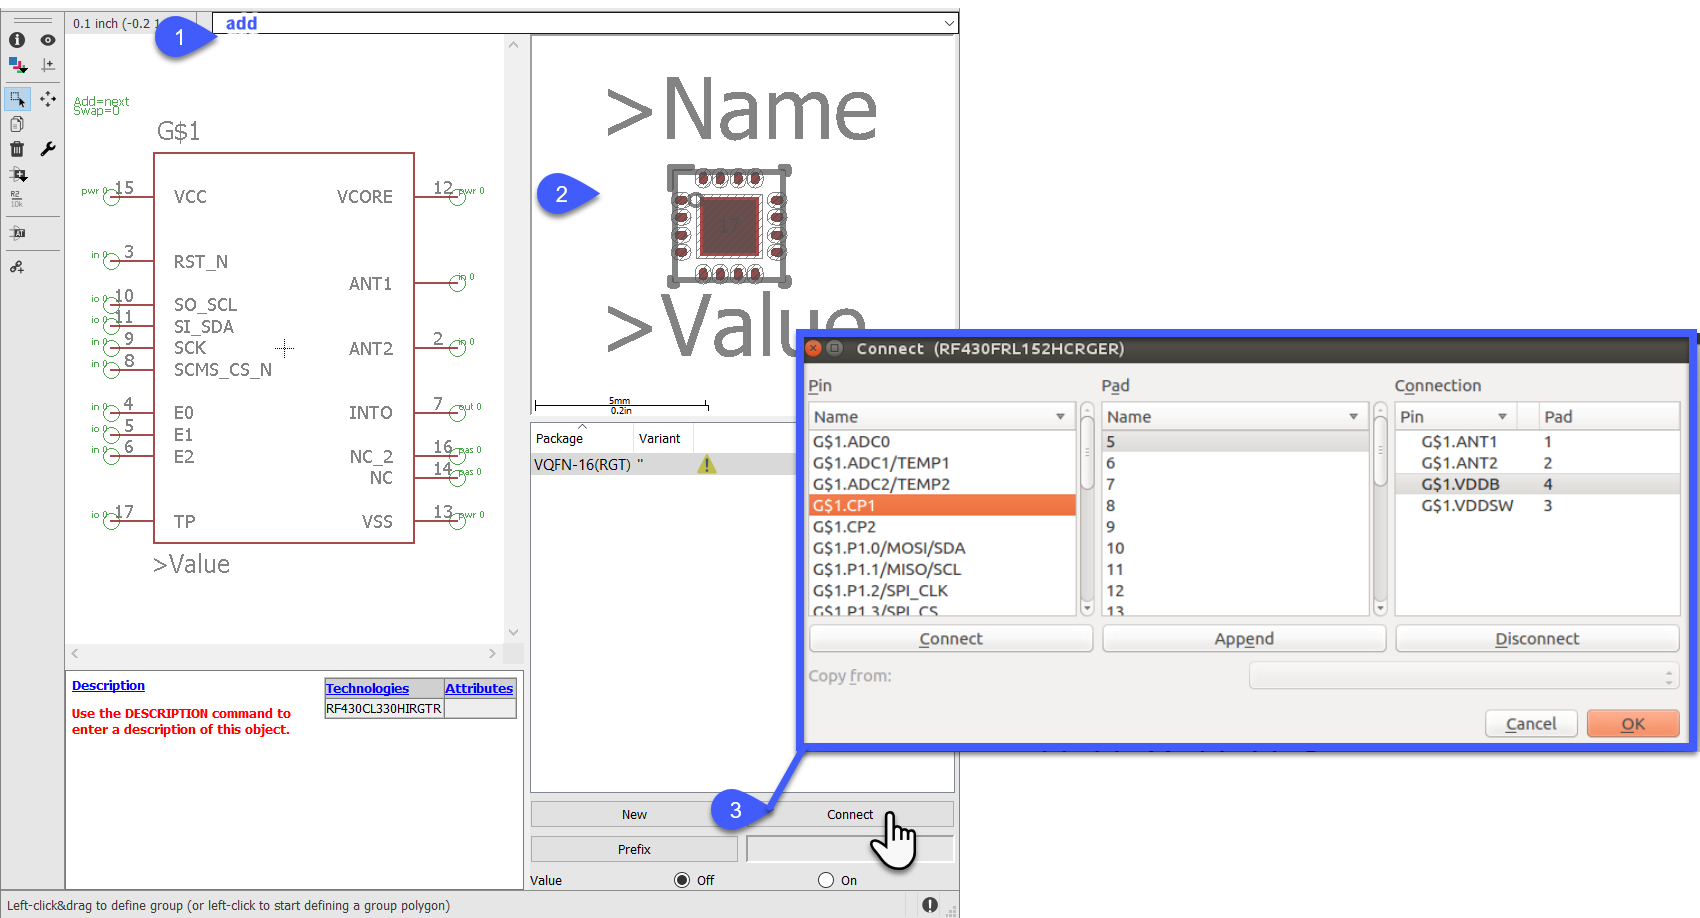
\includegraphics[scale=0.3]{Illustrations/creating_a_device.png}  
\caption{Creating a device in Eagle}
\label{eagle_package}
\end{center}
\end{figure}

\begin{enumerate}
\item Type \textbf{add} and place the symbol.
\item Type \textbf{add} and place the package.
\item Select the package and connect all of the created pins to the corresponding pad. Save the library.
\end{enumerate}


\subsection{ Add an existing device to a managed library }
A library with all necessary component is created. A managed library creates a connection between Eagle and Fusion 360 and is used to create a3D model of the board. The creation of such a library is done as shown in Figure \ref{eagle_fusion}.

The MSP430F2274 chip symbol and footprint were downloaded using Webench \cite{TexasInstruments} and imported into Eagle as shown in Figure \ref{adding_to_library}. 

\begin{figure}[h]
\begin{center}
\center
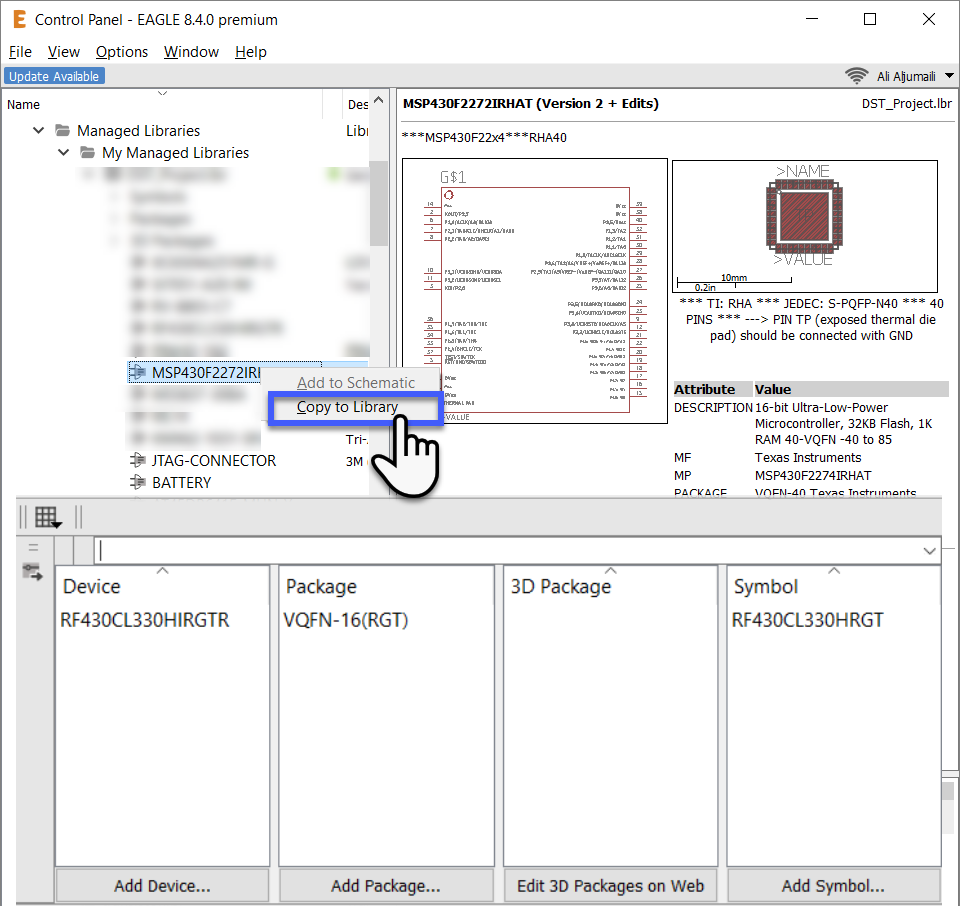
\includegraphics[scale=0.35]{Illustrations/adding_component_to_library.png}  
\caption{Adding an existing component to a library}
\label{adding_to_library}
\end{center}
\end{figure}

\begin{figure}[h]
\begin{center}
\center
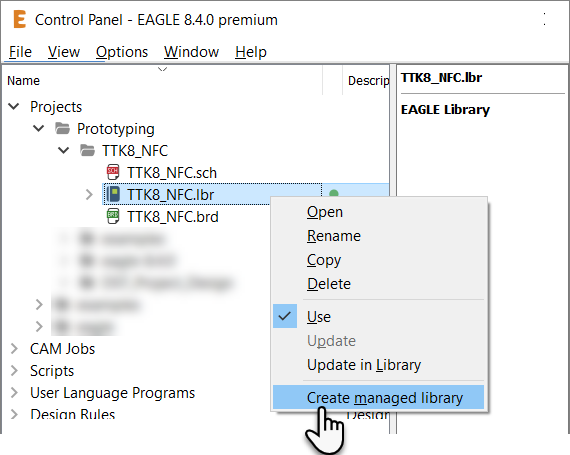
\includegraphics[scale=0.6]{Illustrations/creating_manged_library.png}  
\caption{Creating a manged library library}
\label{eagle_fusion}
\end{center}
\end{figure}



\section{Creating the board outline}
A 2 layer board is developed with the following considerations:
\begin{itemize}
\item 1 oz copper stackup to keep the price to a minimum.
\item Trace width depends heavily on the current, traces carrying high amount of currents should have larger trace width.
\item No right angles in traces, this is to avoid any logical faults in signals where most signals are dependent on edges. 
\item Decoupling capacitors placed as closed to the power pins as possible. 
\item Design check rules to check for air wires and margin faults.
\item No autorouter. This is mainly because the autorouter is terrible, as well to avoid any "antenna" looking routes.
\end{itemize}
Figure \ref{eagle_board} and  shows the final board outline as well to an explanation to what the different layers are.

\begin{figure}[h]
\begin{center}
\center
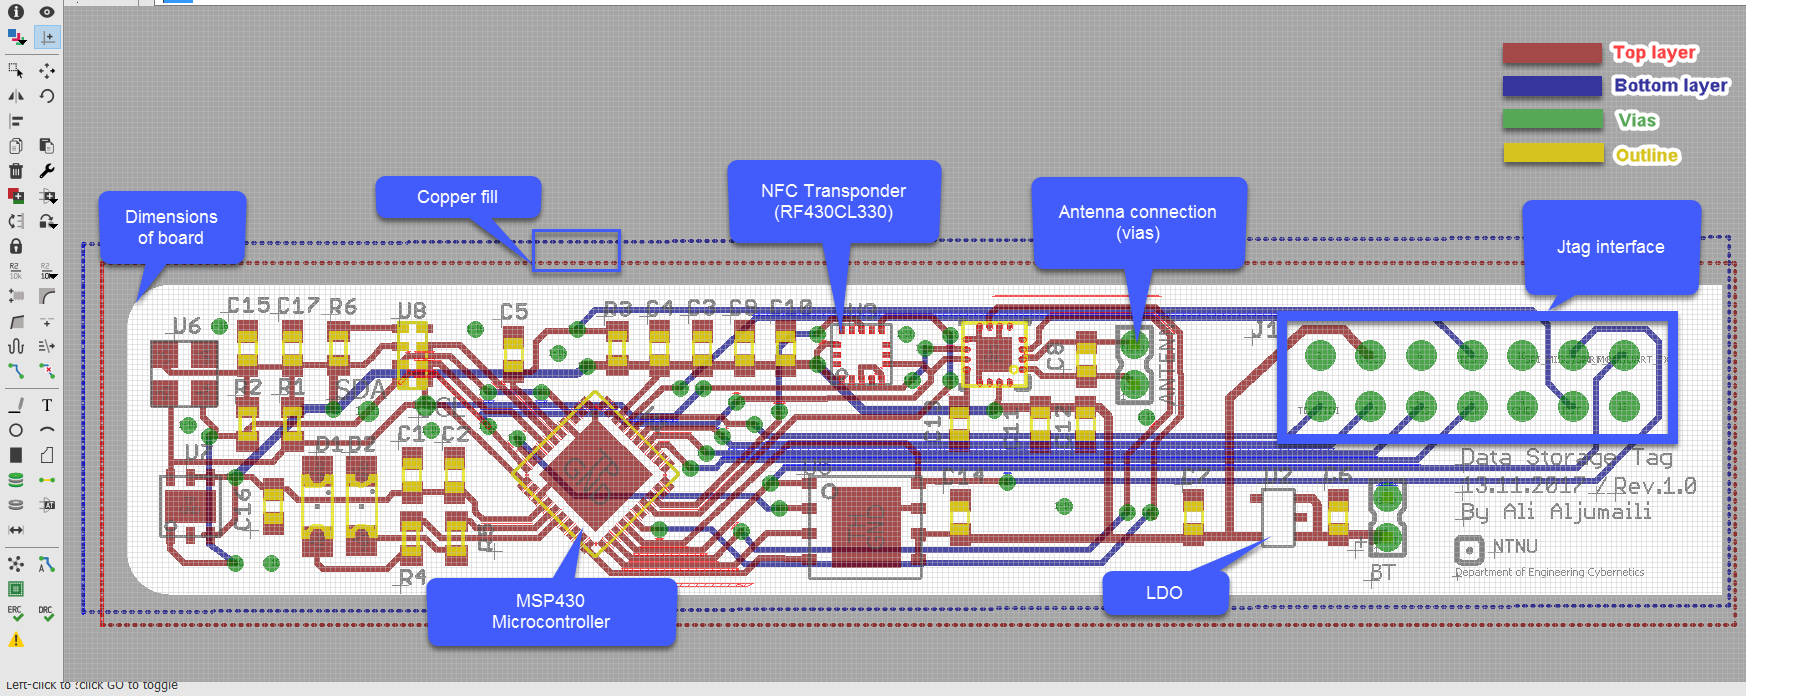
\includegraphics[scale=0.4]{Illustrations/board_explained.png}  
\caption{Board layout explained}
\label{eagle_board}
\end{center}
\end{figure}

\begin{figure}[h]
\begin{center}
\center
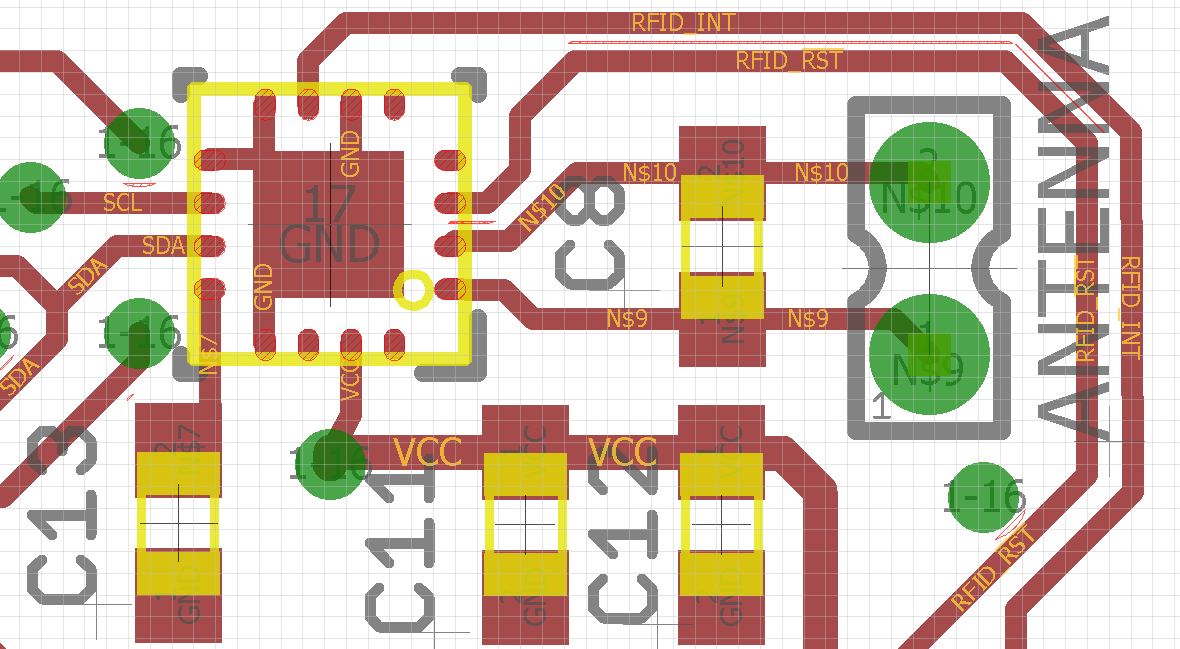
\includegraphics[scale=0.4]{Illustrations/board_only_chip.png}  
\caption{Top board layout for NFC chip}
\label{only_chip}
\end{center}
\end{figure}


\section{Board 3D model}
The managed library can be found by right clicking on the library and choosing view on web. The 3D model is called "Package" in Fusion 360. One must click Edit then choose upload .step to upload the 3D model for the packages. This is done to all of the missing packages as shown in Figure \ref{missing_package}.
\begin{figure}[h]
\begin{center}
\center
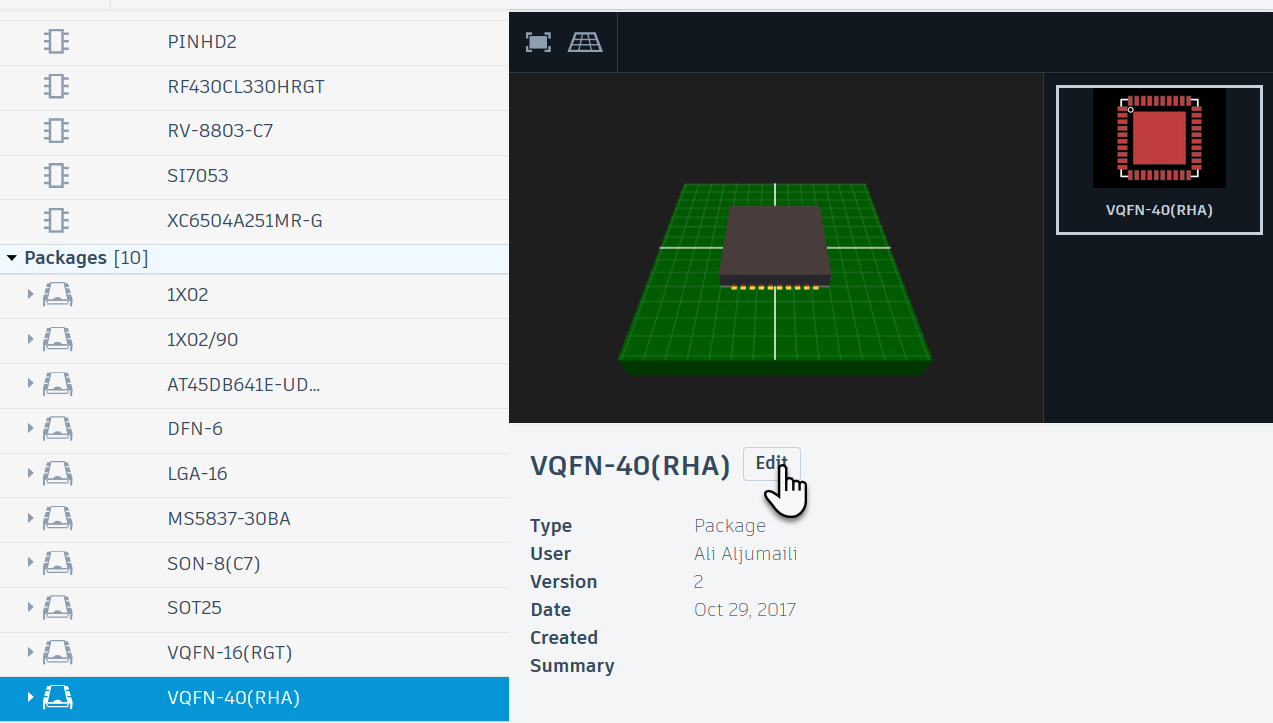
\includegraphics[scale=0.4]{Illustrations/creating_manged_library_edit.png}  
\caption{Adding missing packages}
\label{missing_package}
\end{center}
\end{figure}

\subsection{Generating the 3D model}
The 3D model is generated after updating all of the packages with a .step (3D) package and pushing the board outline from Eagle to Fusion 360 as shown in Figure \ref{pushing_3D}.


\begin{figure}[h]
\begin{center}
\center
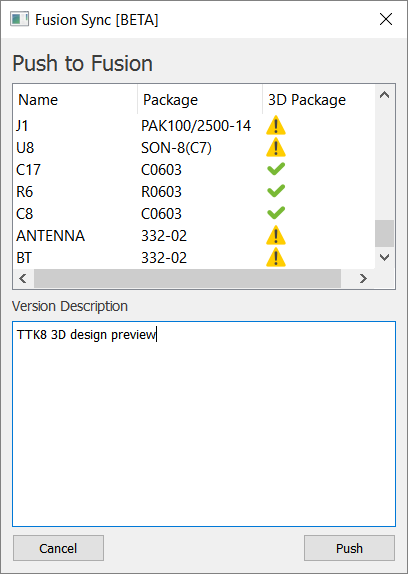
\includegraphics[scale=0.6]{Illustrations/export_fusion.png}   
\caption{Pushing 3D model to Fusion 360}
\label{pushing_3D}
\end{center}
\end{figure}


\section{Eagle Design directory explained}
All of the design files will be found under: \textbf{[Installation-folder]/Eagle-design}
\begin{table}
\centering
\begin{tabular}{|c|c|}
\hline 
\rowcolor{Gray}
File name  & Description  \\ 
\hline 
TTK8-NFC.lbr & Contains an Eagle library with the created components \\ 
\hline 
NFC-Schematics.sch & Contains the schematics for the project \\ 
\hline 
DST-project.brd & Contains the board layout, this is used to generate the gerber files \\ 
\hline 
DST-project.sch & Contains symbols for the corresponding board layout \\ 
\hline 
\end{tabular} 
\caption{Project design files and description} \label{tb:design}
\end{table}
